

\فصل{مقدمه}

چهارپره یا کوادکوپتر\LTRfootnote{Quadcopter} یکی از انواع وسایل پرنده است. چهارپره‌ها نوعی هواگرد بالگردان هستند و در دسته‌ی چندپره‌ها جای دارند.
 %و به‌دلیل کمک گرفتن از چهار پروانه برای نیروی پیشرانش، به عنوان کواد (چهار) کوپتر نامیده می‌شوند. (جمله اضافی)
  چهارپره‌ها به‌دلیل داشتن توانایی مانور خوب و امکان پرواز ایستا با تعادل بالا کاربردهای بسیار گسترده‌ای دارند.
در سال‌های اخیر توجه شرکت‌ها، دانشگاه‌ها و مراکز تحقیقاتی بیش از پیش به این نوع از پهپادها جلب شده‌است. بنابراین، روزانه پیشرفت چشمگیری
%  اسم فاعل سر هم%
 در امکانات و پرواز این نوع از پرنده‌ها مشاهده می‌کنیم. چهارپره‌ها در زمینه‌های تحقیقاتی، نظامی، تصویربرداری، تفریحی و کشاورزی کاربرد زیاد و روزافزونی دارند و مدل‌های دارای سرنشین آن نیز تولید شده‌است‌.





\قسمت{تاریخچه}
مدل‬ اولیه آزمایشی یک چندپره در سال ۱۹۰۷ توسط دو برادر فرانسوی بنام
 \lr{Jacques} و \lr{Louis Breguet}
  ساخته‌شد. پرنده آن‌ها موفق به پرواز به‌صورت عمودی شد؛ ولی تنها تا ارتفاع دو فوتی پرواز کرد. پرواز انجام شده یک پرواز آزاد\LTRfootnote{Free Flight}
  نبود و پرنده به کمک چهار مرد ثابت نگه‌داشته شده‌بود \cite{Sprekelmeyer}.
  بعد از آن ساخت بالگرد چهار پروانه‌ای به سال ۱۹۲۰ میلادی برمی‌گردد. در آن سال یک مهندس فرانسوی به نام \lr{Étienne Oehmichen} اولین بالگرد چهارپره را اختراع کرد و مسافت ۳۶۰ متر را با چهارپره خود پرواز کرد. در همان سال او مسافت یک کیلومتر را در مدت هفت دقیقه و چهل ثانیه پرواز کرد \cite{10.2307/44729509}.

در  سال ۱۹۲۲ در آمریکا \lr{George de Bothezata} موفق به ساخت و تست تعدادی چهارپره برای ارتش شد که قابلیت کنترل و حرکت در سه بعد را داشت، ولی پرواز با آن بسیار سخت بود.

در سال‌های اخیر توجه مراکز دانشگاهی به طراحی و ساخت پهپادهای چهارپره جلب شده‌است و مدل‌های مختلفی در دانشگاه استنفورد و کورنل ساخته شده‌است و به تدریج رواج یافته‌است~\cite{5717652}.
از حدود سال ۲۰۰۶ کواد کوپترها شروع به رشد صنعتی به‌صورت وسایل پرنده بدون سرنشین نمودند.


\قسمت{تعریف مسئله}
مسئله‌ای که در این پروژه بررسی می‌شود، کنترل وضعیت سه درجه آزادی استند آزمایشگاهی چهارپره با استفاده از روش کنترل مربعی خطی انتگرالی مبتنی بر بازی دیفرانسیلی است. این استند آزمایشگاهی (شکل \ref{LabQuad1}) شامل یک چهارپره است که از 
مرکز توسط یک اتصال به یک پایه وصل شده‌است. در این صورت، تنها وضعیت چهارپره (زوایای رول\LTRfootnote{Roll}، پیچ\LTRfootnote{Pitch} و یاو\LTRfootnote{Yaw}) 
 تغییر کرده و فاقد حرکت انتقالی است. همچنین، می‌توان با مقیدکردن چرخش حول هر محور، 
حرکات رول، پیچ و یاو  پرنده را به‌صورت مجزا و یا با یکدیگر بررسی کرد.

\begin{figure}[H]
	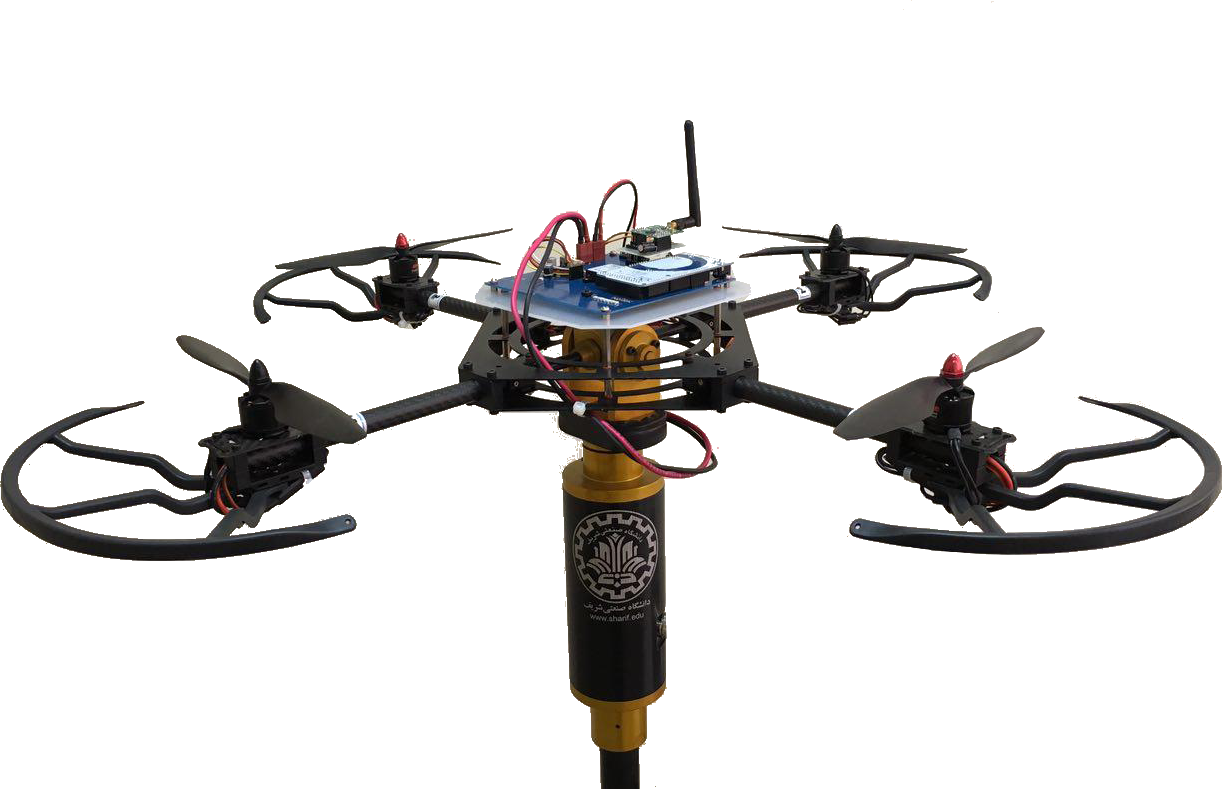
\includegraphics[width=12cm]{../Figures/introduction/3DOFQuad.png}
	\centering
	\caption{استند کنترل وضعیت سه درجه آزادی چهارپره 
	\cite{Iranlabexpo}}
\label{LabQuad1}
\end{figure}
با توجه به شکل
\ref{LabQuad1}،
مرکز جرم این استند بالاتر از مفصل قرار دارد که می‌توان آن را به‌صورت آونگ معکوس در نظر گرفت. بنابراین، سامانه به‌صورت حلقه‌باز ناپایدار است. این سامانه دارای چهار ورودی مستقل (سرعت چرخش پره‌ها) و سه خروجی زوایای اویلر
$(\psi ,\theta ,\phi)$
است. در مدل‌سازی این استند عدم قطعیت وجود دارد; اما، با توجه به کنترل‌کننده مورد استفاده می‌توان این عدم قطعیت را به‌صورت اغتشاش درنظر گرفت و سامانه را به خوبی کنترل کرد. 
%در پایان، با کنترل‌کننده
% تنظیم‌کننده مربعی خطی\LTRfootnote{LQR (Linear Quadratic Regulator)} مقایسه خواهد ‌شد.


%\subsection{ساختار بالگرد}
%
%بالگرد‌ها همانند انواع دیگر وسایل پرنده از ایجاد اختلاف فشار در اتمسفر پیرامون خود و ایجاد نیروی برآ\LTRfootnote{Lift} برای بلندشدن و حرکت در هوا استفاده می‌کنند. به‌دلیل وجود نیروی عمل و عکس‌العمل در بالگردها، پس از اینکه پره اصلی شروع به چرخش می‌کند، با برخورد مولکول‌های هوا به این پره و وجود عکس‌العمل، یک نیرویی با جهت مخالف جهت چرخش پره به پره و در ادامه گشتاوری به شفت متصل به پره اعمال می‌شود و این گشتاور باعث چرخش بالگرد به دور خود می‌شود. در بالگرد برای حل این مشکل، از پره دم استفاده می‌شود تا گشتاوری را تولید کند که مانع چرخش بالگرد به دور خود شود. 
%\begin{figure}[H]
%	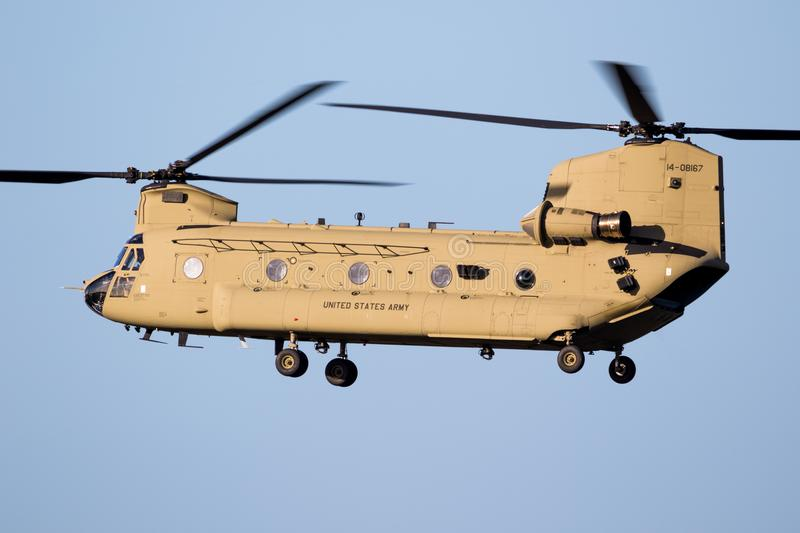
\includegraphics[width=10cm]{../Figures/introduction/boeing-ch-chinook.jpg}
%	\centering
%	\caption{بالگرد شینوک
%		\cite{CH-47}}
%	\label{chinook}
%\end{figure}
%حال اگر بالگرد به جای داشتن یک پره اصلی از دو پره اصلی که خلاف جهت یکدیگر بچرخند استفاده می‌نمود، به‌دلیل خنثی‌شدن دو  گشتاور توسط یکدیگر، دیگر بالگرد به دور خود نمی‌چرخید. مانند بالگردهای شینوک\LTRfootnote{Boeing CH-47 Chinook} که نمایی از آن در شکل
%\ref{chinook}
%آورده شده‌است. حال، با توجه به توضیحات داده‌شده، راحت‌تر می‌توان به ساختار چهارپره‌ها اشاره نمود.
%\subsection{ساختار چهارپره}


چهارپره‌ها با بهره‌گیری از چهار موتور و پره مجزا و چرخش دو به دو معکوس این موتورها، گشتاورهای عکس‌العملی یکدیگر را خنثی می‌کنند و همچنین اختلاف فشار لازم جهت ایجاد نیروی برآ را تأمین می‌کنند.

\begin{figure}[H]
	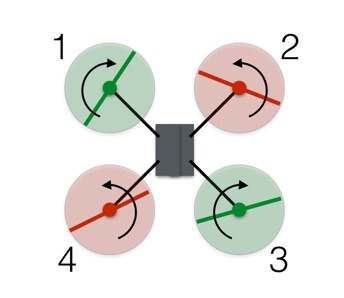
\includegraphics[width=8cm]{../Figures/introduction/Quadblade.jpg}
	\centering
	\caption{جهت چرخش پره‌های چهارپره
		\cite{Quadhowfly}}
\end{figure}

نحوه ایجاد فرامین کنترلی در چهارپره‌ها به این صورت است که برای تغییر ارتفاع از کم یا زیاد کردن سرعت چرخش موتورها استفاده می‌شود و باعث کم یا زیاد شدن نیروی برآ می‌شود. برای چرخش چهارپره به دور خود و به‌صورت درجا، دو پره هم جهت با سرعت کمتر و دو پره هم جهت دیگر با سرعت بیشتر می‌چرخند و گشتاور یاو ایجاد می‌شود و نیروی برآ ثابت می‌ماند؛
%(زیرا دو پره با سرعت کمتر و دو پره دیگر به همان نسبت با سرعت بیشتر می‌چرخند.)
 بنابراین، چهارپره در ارتفاع ثابت به دور خود می‌چرخد. همچنین، با کم و زیاد کردن دو به دو سرعت موتورهای مجاور چهارپره از حالت افقی خارج شده و در صفحه افق حرکت می‌کند.


\section{نظریه بازی}
نظریه بازی با استفاده از مدل‌های ریاضی به تحلیل روش‌های همکاری یا رقابت موجودات منطقی و هوشمند می‌پردازد. نظریه بازی، شاخه‌ای از ریاضیات کاربردی است که در علوم اجتماعی و به ویژه در اقتصاد، زیست‌شناسی، مهندسی، علوم سیاسی، روابط بین‌الملل، علوم رایانه، بازاریابی و فلسفه مورد استفاده قرار می‌گیرد. نظریه بازی در تلاش است تا به وسیله‌ی ریاضیات، رفتار را در شرایط راهبردی یا در یک بازی که در آن موفقیت فرد در انتخاب کردن، وابسته به انتخاب دیگران می‌باشد، برآورد کند.
\subsection{تاریخچه نظریه بازی}
%در سال ۱۹۲۱ یک ریاضی‌دان فرانسوی به نام اِمیل بُرِل برای نخستین بار به مطالعهٔ تعدادی از بازی‌های رایج در قمارخانه‌ها پرداخت و چند مقاله در موردِ آن‌ها نوشت. او در این مقاله‌ها بر قابل پیش‌بینی بودنِ نتایجِ این نوع بازی‌ها از راه‌های منطقی، تأکید کرده بود. 
%کوتاه است یا نه؟؟؟؟؟؟؟؟؟؟؟
در سال ۱۹۹۴ جان فوربز نش به همراه جان هارسانی و راینهارد سیلتن به خاطر مطالعات خلاقانه‌ی خود در زمینه‌ی نظریه بازی، برنده‌ی جایزه نوبل اقتصاد شدند. در سال‌های پس از آن نیز بسیاری از برندگان جایزه‌ی نوبل اقتصاد از میان متخصصین نظریه بازی انتخاب شدند. آخرین آن‌ها، ژان تیرول فرانسوی است که در سال ۲۰۱۴ این جایزه را کسب کرد \cite{nobel}.
\subsection{تعادل نش}
پژوهش‌ها در این زمینه اغلب بر مجموعه‌ای از راهبردهای شناخته شده به عنوان تعادل در بازی‌ها استوار است. این راهبردها به‌طور معمول از قواعد عقلانی به نتیجه می‌رسند. مشهورترین تعادل‌ها، تعادل نش است. 
تعادل نش در بازی‌هایی کاربرد دارد  در آن فرض شده‌است که هر بازیکن به راهبرد تعادل دیگر بازیکنان آگاه است.
%در نظریه بازی، تعادل نش (به نام جان فوربز نش، که آن را پیشنهاد کرد) راه حلی از نظریه بازی است که شامل دو یا چند بازیکن است، که در آن فرض بر آگاهی هر بازیکن به راهبرد تعادل دیگر بازیکنان است. 
بر اساس نظریه‌ی تعادل نش، در یک بازی که هر بازیکن امکان انتخاب‌های گوناگون دارد اگر بازیکنان به روش منطقی  راهبردهای خود را انتخاب کنند و به دنبال حداکثر سود در بازی باشند، دست کم یک راهبرد برای به دست آوردن بهترین نتیجه برای هر بازیکن وجود دارد و چنانچه بازیکن راهکار دیگری را انتخاب کند، نتیجه‌ی بهتری به دست نخواهد آورد.



